% nakagawa_thesis.tex
% ーーーーーーーーーーーーーーーーーーーーーーーーーーーーーーー

\documentclass[a4paper,12pt]{article_vdlab_sotsuron}
\pagestyle{plain}

\usepackage{setspace}
\usepackage{graphicx}
\usepackage{amsmath,amssymb}
\usepackage{colortbl}
\usepackage{comment}

\begin{document}
%文字間隔を設定
\kanjiskip = .0pt plus 3pt minus 3pt
\xkanjiskip = .0pt plus 3pt minus 3pt
\small
\setstretch{1.5}

% ーーーーーーーーーーーーーーーーーーーーーーーーーーーーーーー

\begin{center}
  % 論文題目
  \jtitle{IDCS制御手法を用いたHILSシステムの検討}
  \etitle{Investigation of HILS system using IDCS}
\end{center}

%目次の表示
\tableofcontents

% ーーーーーーーーーーーーーーーーーーーーーーーーーーーーーーー

\newpage
\section{序論}
\subsection{タイヤとサスペンション}
タイヤは自動車において唯一路面と接触する要素であり,自動車の基本的な機能である「走る」「曲がる」「止まる」といった運動は,すべて路面とタイヤとの間に発生する摩擦力によって実現している.そのため,タイヤは車両運動に直接影響を与える重要なようであると言える.したがって,タイヤの特性を十分理解することで車両の運動特性を把握し,その性能を十分に発揮させることができる.タイヤの状態に影響を及ぼす要因として,車体とタイヤを連結するサスペンション機構が挙げられる.車体重量を支持すると共に,車輪の上下振動を緩和,吸収して,振動が車体に直接伝達されることを防止する.また,路面間に発生する駆動力,制動力,横力など各種の路面反力を車体に伝達することで,車両運動性能に影響を与える.したがって,車両運動特性を把握するためには,タイヤとサスペンションを複合的に評価する必要がある.
% ーーーーーーーーーーーーーーーーーーーーーーーーーーーーーーー
% suspension
%  ーーーーーーーーーーーーーーーーーーーーーーーーーーーーーーー

\vspace{10mm}
\begin{figure}[h!]
  \begin{tabular}{cc}
    \begin{minipage}{1.0\hsize}
      \begin{center}
	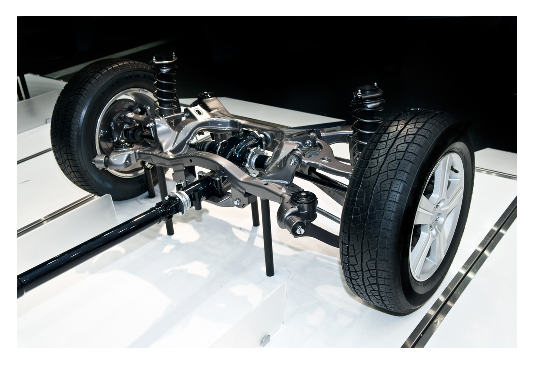
\includegraphics[scale = 1.0]{figure/pic_suspension.eps}
	\caption{Suspension System\cite{pic_sus.net}}
	\label{fig:suspension}
      \end{center}
     \end{minipage}
    \end{tabular}
\end{figure}

% ーーーーーーーーーーーーーーーーーーーーーーーーーーーーーーー
\newpage
\subsection{Hardware-in-the-Loop Simulation(HILS)システム}
車両運動性能を車両運動性能を評価する手法として,シミュレーションや実写走行試験などが挙げられる.しかし,シミュレーションでは,評価対象のモデル化誤差が障子,実写走行試験では,同一条件での試験が困難である.このような問題を解決するシステムとしてHILSシステムが用いられている\cite{exp_hils1}.HILSとはHardware-in-the-Loop Simulationの略であり,リアルタイムシミュレーションを用いたシステム評価手法である.解析で得た値を目標値として実機を動かし,実機を動かす子によって得た計測値を用いて解析を行う.従来の時刻歴シミュレーションと実機試験のそれぞれの欠点を補完するようなものとなり,シミュレーション精度の向上を図りながら,試験に必要なコストを抑え,試験の自由度を確保することができる.このため,部品開発の一段階としてHILSを導入することで,制度と効率の両面において質の高い試験が可能となり,開発の大幅な効率化が期待できる\cite{exp_hils2}.

% ーーーーーーーーーーーーーーーーーーーーーーーーーーーーーーー
% hils
%  ーーーーーーーーーーーーーーーーーーーーーーーーーーーーーーー

\vspace{10mm}
\begin{figure}[h!]
  \begin{tabular}{cc}
    \begin{minipage}{1.0\hsize}
      \begin{center}
	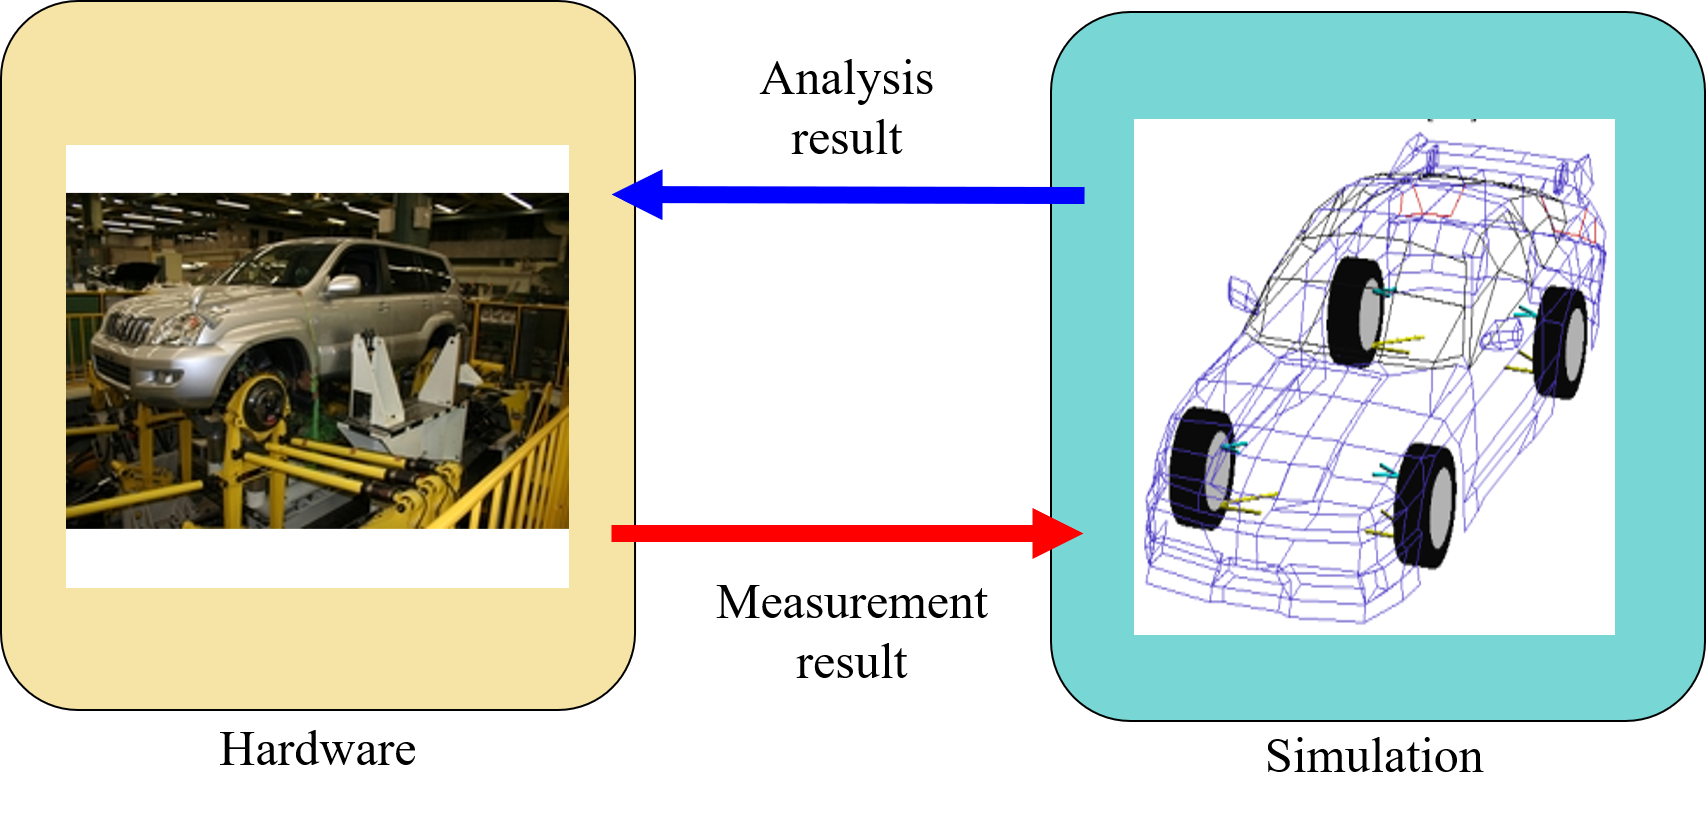
\includegraphics[scale = 0.4]{figure/hils.eps}
	\caption{HILS System\cite{toyota_hils}}
	\label{fig:HILS system}
      \end{center}
     \end{minipage}
    \end{tabular}
\end{figure}

% ーーーーーーーーーーーーーーーーーーーーーーーーーーーーーーー
\subsection{研究目的}
前述のように,HILSシステムは試験機の計測結果を用いた解析を行い,その解析結果に基づいて試験機のアクチュエータの入力を決定し特性評価を行うシステムである.HILSシステムはシミュレーション解析と実機試験の同期が必要であるため,高い制御精度が求められる.

そこで本研究では,HILSシステムの再現性の向上を目的として,IDCSと呼ばれる制御手法を用いHILSシステムの制御精度の向上を行った.研究室で開発したHILS試験機を用いて,試験機の挙動と解析結果を比較することで,IDCSの有効性を検証した.また路面-車体間の相対変位を用いる制御手法による解析結果と,IDCSによる解析結果を比較し,IDCSによる制御の優位性を確認した.


% -------------------------------------
\newpage
\section{HILSシステムの構成}
\subsection{タイヤ―サスペンションHILSシステム}
本研究で用いるタイヤ―サスペンションHILSシステムの概要を図~\ref{fig:tier-suspension HILS}~に示す.タイヤーサスペンションHILSシステムとは,計測値を用いたシミュレーション解析を行うソフトウェア部と,解析値を用いて実機試験を行うハードウェア部から構成される.本システムでは試験装置から計測されたダンパ力を用いてリアルタイムに車両運動解析を行い,ばね上ーばね下間相対変位を算出する.この解析結果に基づきアクチュエータの入力を決定し,リアルタイムに車両の上下動を再現している.

% HILSの概要図-------------------------------
\vspace{20mm}
\begin{figure}[h]
  \begin{center}
  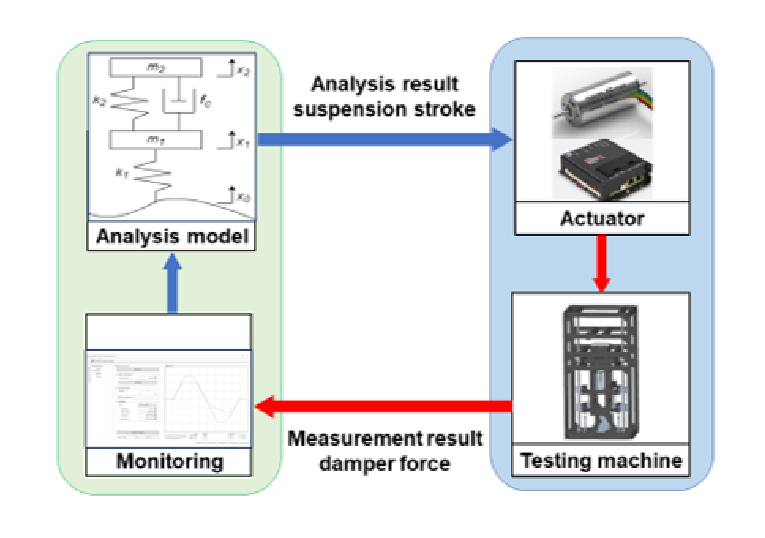
\includegraphics[height=80mm]{figure/HILS_loop.eps}
  \vspace{4mm}
   \caption{Tire-Suspension HILS System}
  \label{fig:tier-suspension HILS}
  \end{center}
\end{figure}

\newpage
\subsection{ハードウェア}
\subsubsection{HILS試験機}

本研究で用いるHILS試験機を図~\ref{fig:HILS_machine}~に示す.この装置は上下1自由度で,自動車の車体をばね上で,タイヤ-サスペンション系をばね下とばね・ダンパで表現している.また路面部にはアクチュエータを取り付けている.

ソフトウェア部で行う解析によって得たサスペンションストロークをばね上ばね下間の変位として実現している.またレーザ変位計とロードセルを用いて,サスペンションストロークとダンパ力を計測しており,ダンパ力はソフトウェア部の解析に用いられる.


% HILS_machine ---------------------------
\vspace{20mm}
\begin{figure}[h]
  \begin{center}
  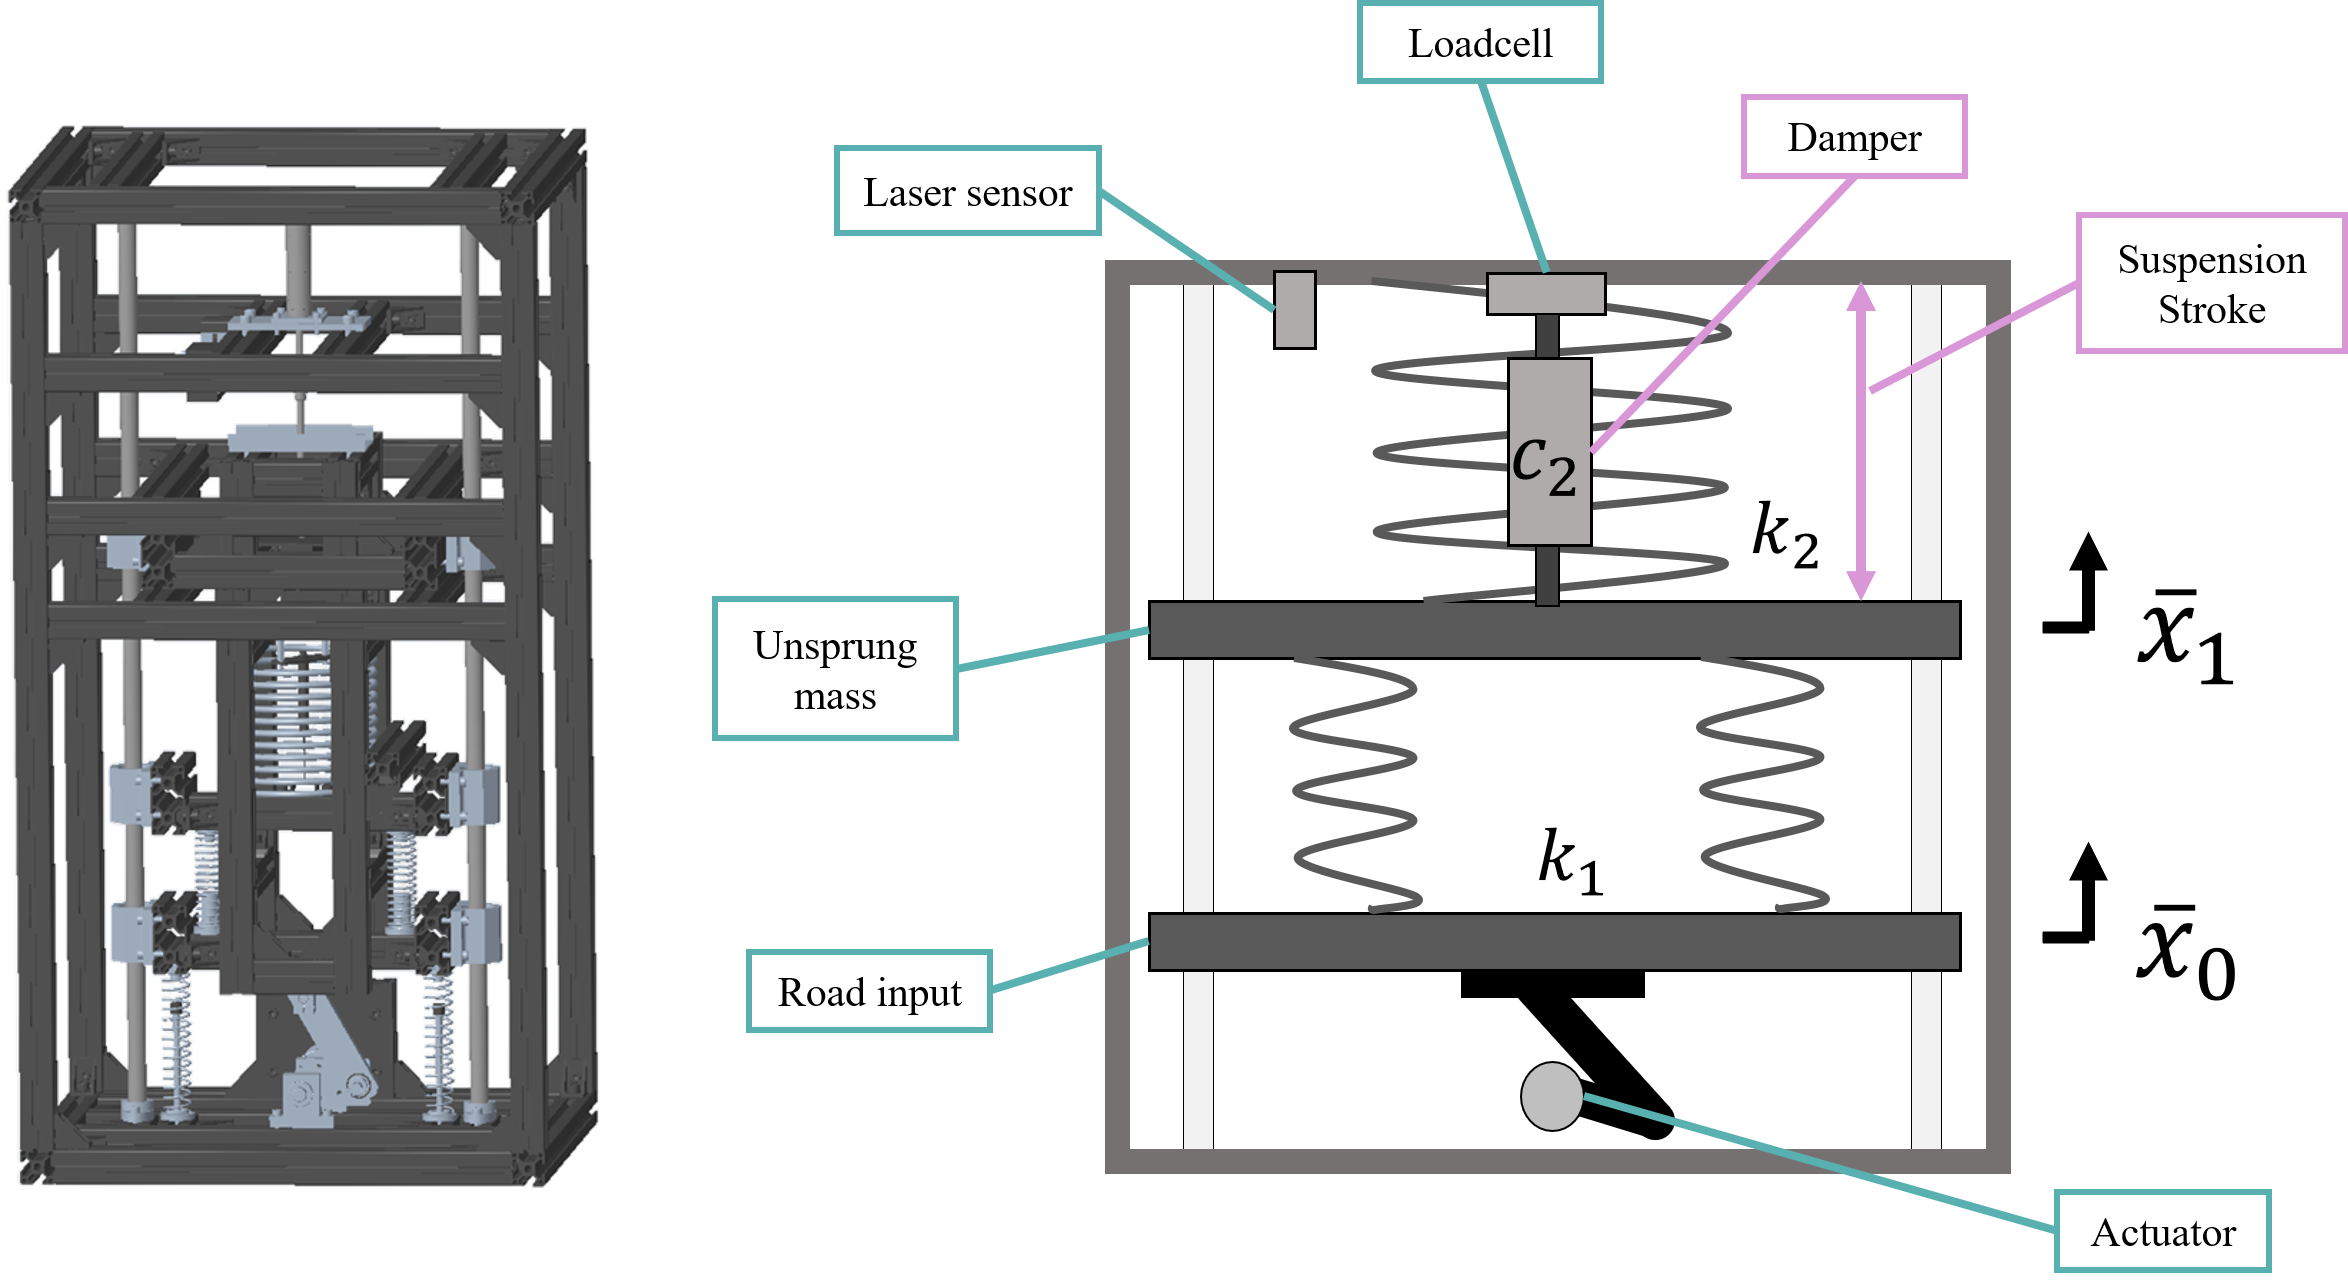
\includegraphics[height=80mm]{figure/HILS_machine.eps}
  \vspace{4mm}
   \caption{HILS Testing Machine}
  \label{fig:HILS_machine}
  \end{center}
\end{figure}

\newpage
\subsubsection{アクチュエータ}
本試験機の路面部入力を行うアクチュエータにはモータを用いる.そのモータの特性と制御ユニットとして用いるモータドライバについて説明する.

本試験機に用いるアクチュエータはmaxon$\ $japan株式会社のECモータ「EC-max$\ $40$\ $283867」である.モータの外観を図~\ref{}~に,モータスペックを表~\ref{tab:ecmax40}~に示す.モータの先端にはギアヘッドが取り付けてあり,回転方向や角度を検出する電子部品としてエンコーダが取り付けられている.このモータにはmaxon$\ $japan株式会社のブラ寝たりギアヘッド「GP42C$\ $203126」とエンコーダ「HEDL55405540$\ $115016」を取り付けた.それぞれの仕様を表~\ref{tab:Gearhead}~,表~\ref{tab:Encoder}~に示す.

% アクチュエータ性能----------------------
\vspace*{10mm}
\begin{figure}[htp]
  \begin{minipage}{0.4\textwidth}
    \begin{center}
      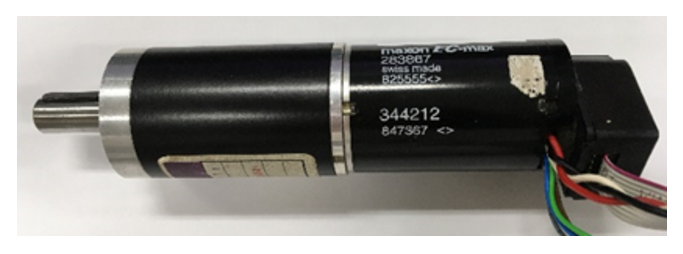
\includegraphics[height=20mm]{figure/ecmax40.eps}
      \vspace*{3mm}
      \caption{ECmax40 283867}
      \label{fig:ecmax40}
    \end{center}
  \end{minipage}
  \begin{minipage}{0.6\textwidth}
      \begin{center}
	\makeatletter
	\def\@captype{table}
	\makeatother
	\caption{Specification of EC Servomotor(283867)}
	\label{tab:ecmax40}
	  \begin{tabular}{cc}\hline
	    Nominal output & 70 [W] \\
	    Nominal voltage & 24 [V] \\
	    Nominal speed & 12000 [rpm] \\
	    Max continuous Torque & 89.6 [mNm] \\
	    Max continuous current & 3.44 [A] \\
	    Torque constant & 28 [mNm/A] \\
	    Speed constant & 341 [rpm/V] \\\hline
	  \end{tabular}
	\end{center}
  \end{minipage}
\end{figure}

\vspace*{10mm}
\begin{table}[htp]
  \begin{minipage}{0.5\textwidth}
    \begin{center}
      \makeatletter
	\def\@captype{table}
	\makeatother
	\caption{Specification Gearhead(203126)}
	\label{tab:Gearhead}
	  \begin{tabular}{cc}\hline
	    Gear Ratio & 113:1 \\
	    Rated speed & 8000 [rpm] \\
	    Backlash & 1.0 [deg] \\
	    Max continuous torque & 15 [Nm] \\\hline
	  \end{tabular}
    \end{center}
  \end{minipage}
  \begin{minipage}{0.5\textwidth}
      \begin{center}
	\makeatletter
	\def\@captype{table}
	\makeatother
	\caption{Specification of Encoder(110516)}
	\label{tab:Encoder}
	  \begin{tabular}{cc}\hline
	    Encoder Resolution & 500 [count/rev] \\
	    Max frequency & 100 [kHz] \\
	    Allowable maximum speed & 12000 [rpm] \\\hline
	  \end{tabular}
	\end{center}
  \end{minipage}
\end{table}

\newpage
\subsubsection{モータドライバ}
次にモータドライバについて説明する.先ほどのモータの制御ユニットとして,maxon$\ $japan株式会社の「EPOS$\ $70/10$\ $375711」を使用した.モータドライバの外観を図~\ref{fig:epos}~に,仕様を表~\ref{tab:epos}~に示す.EPOS2は,インクリメンタル・エンコーダ付きDCモータおおyびEC(ブラシレス)モータを駆動可能なデジタル制御ユニットである.CANopen, USB2.3/3.0,RS232通信による通信を可能とし,Point$\ $to$\ $Pointの位置制御,回転数制御,トルク制御を行うことができる.EPOS2$\ $70/10は,モジュール式のデジタル位置制御ユニットで,80~700Wまでのエンコーダ付きんDCモータ,またはホールセンサ/エンコーダ付きブラシレスECモータに対応している.本研究では,RS232通信を用いて位置指令を行い,「Position$\ $Mode」を用いた位置制御によりモータを制御している.電源電圧の供給には,図~\ref{fig:rs_150_24}~に示すMEAN$\ $WELL社のスイッチング電源「RS-150-24」を使用した.

\vspace*{20mm}
\begin{figure}[htp]
  \begin{minipage}{0.4\textwidth}
    \begin{center}
      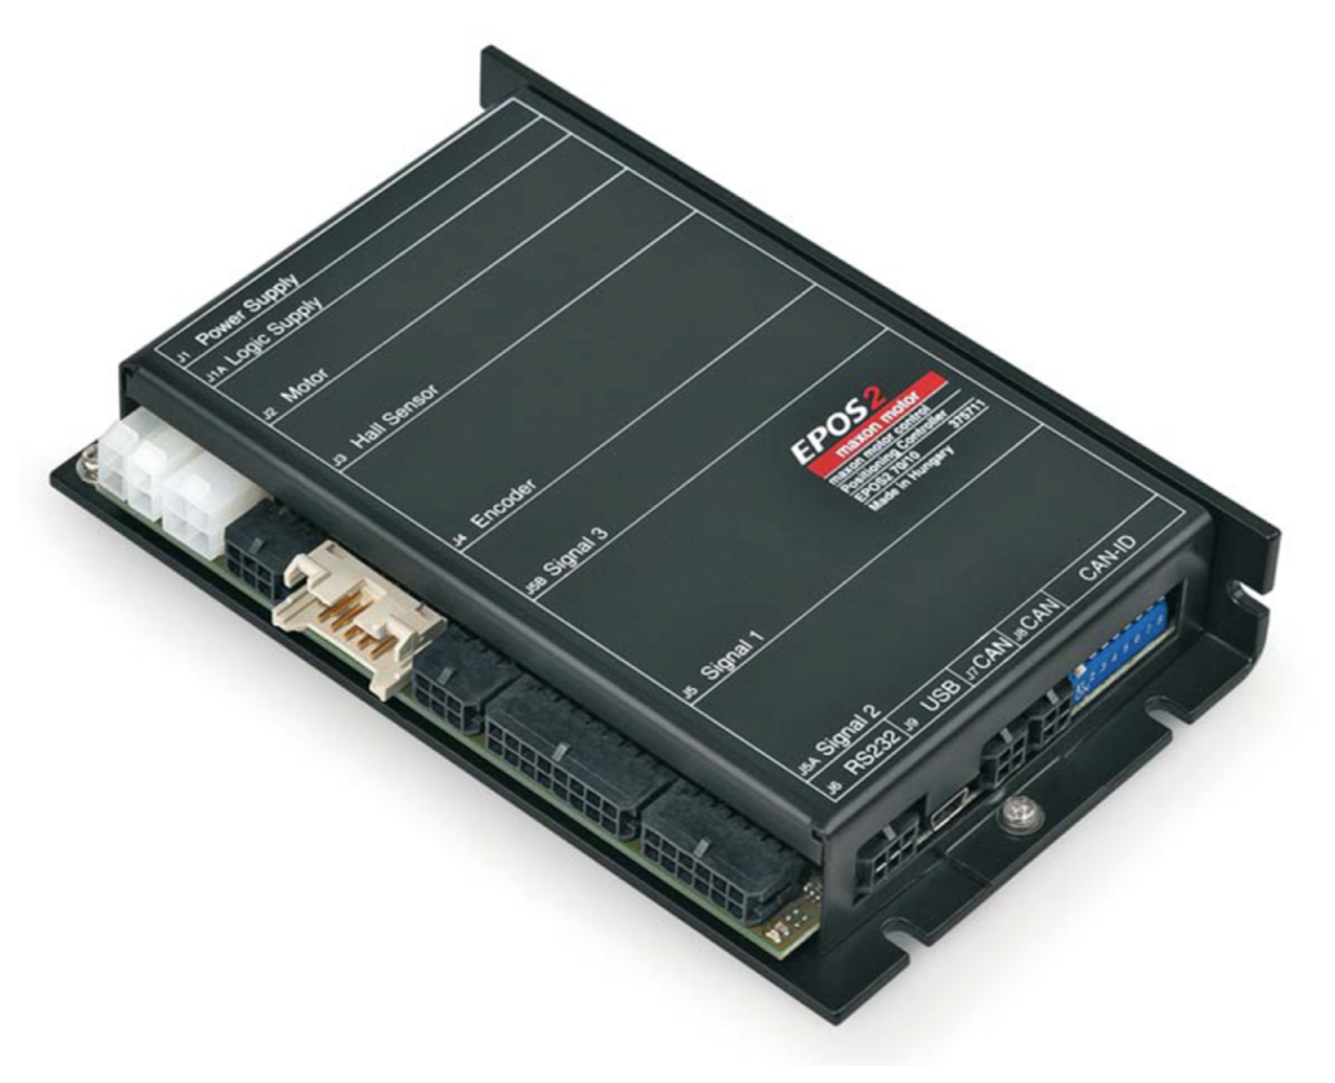
\includegraphics[height=40mm]{figure/epos.eps}
      \vspace*{3mm}
      \caption{EPOS2 70/10(375711)}
    \label{fig:epos}
    \end{center}
  \end{minipage}
  \begin{minipage}{0.6\textwidth}
      \begin{center}
	\makeatletter
	\def\@captype{table}
	\makeatother
	\caption{Specification of EPOS2 70/10(375711)}
	\label{tab:epos}
	\begin{tabular}{cc}\hline
	  power suppy voltage [VDC] & 11-70\\
	  Max output current [A] & 25\\
	  Max continuous current [A] & 10\\
	  Hall sensor & H1, H2, H3 \\
	  Encoder & A, A$\setminus$, B, B$\setminus$, I, I$\setminus$(max. 5MHz)\\
	  Analog Input & 2(differential, 12-bit, 0...+5 V)\\
	  RS232 & RxD; TxD(max. 115200 bit/2) \\\hline
	  \end{tabular}
	\end{center}
  \end{minipage}
\end{figure}

\vspace*{20mm}
\begin{figure}[htp]
  \begin{center}
    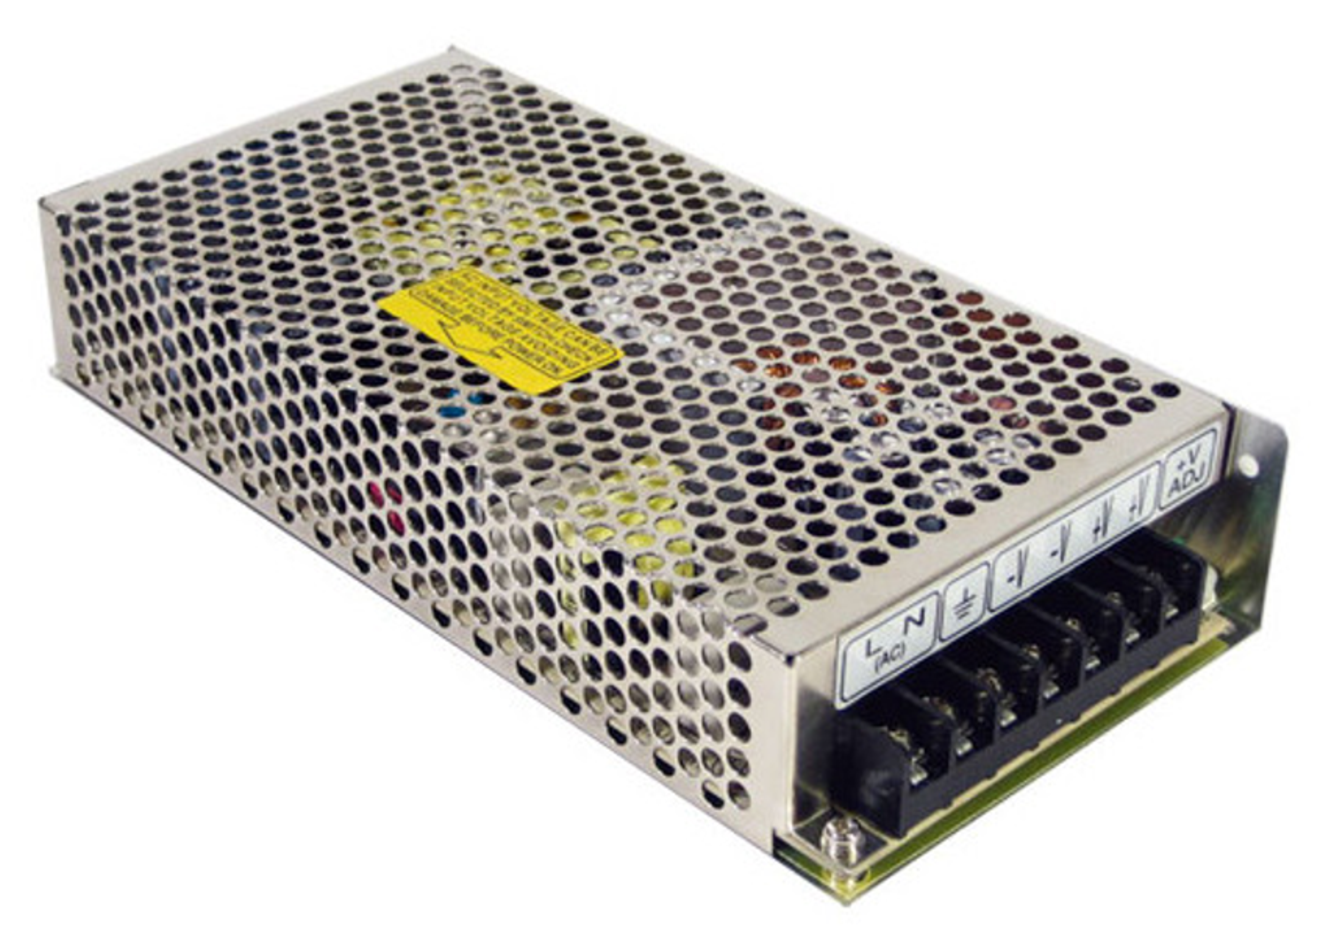
\includegraphics[height=40mm]{figure/rs_150_24.eps}
    \vspace*{3mm}
    \caption{Swiching Power Supply(RS-150-24)}
    \label{fig:rs_150_24}
  \end{center}
\end{figure}


\newpage
本研究では,シリアル通信を用いた位置制御を行った.

\newpage
\subsubsection{スライダクランク機構}
スライダクランク機構は回転運動を直進運動に変換する機構の一つである.図~\ref{fig:slider_crank}~に示すようにクランクとコネクティングロッドから構成される.本研究では路面の変位を$\pm 30mm$確保するためにクランク長は$r=45mm$,コネクティングロッドの長さは$l=90mm$とした.クランクの回転角$\theta_A$とコネクティングロッド先端の変位$x_0$の関係は式(~\ref{eq:mm_to_deg}~)で表される.本研究で行う試験では路面入力を行う為に入力を変位$x_0$,出力を回転角$\theta_A$とする関係式が必要である.しかし式(~\ref{eq:mm_to_deg}~)では計算が複雑である.そこでLook up tableを用いた.Look up tableは予め計算できるデータを配列として格納しておくことで,配列に対応する値を参照してデータを得ることができ,これにより計算の効率化を可能とする.使用したsimulinkブロックを図~\ref{fig:suspension}~に示す.本研究では.Lookuptableの配列データの数は91とした.配列の要素であるクランクの回転角$\theta_A$の範囲は$\pm45[^\circ ]$であり,$0.1[^\circ ]$刻みとした.また変位$x_0$は式(~\ref{eq:mm_to_deg}~)より計算した値となっている.

\begin{equation}
 \label{eq:mm_to_deg}
x_{0} =r\times \sin \theta _{A} +\sqrt{l^{2} -r^{2}\cos^{2} \theta _{A}} -\sqrt{l^{2} -r^{2}}
\end{equation}

\vspace*{5mm}
\begin{figure}[htp]
  \begin{center}
    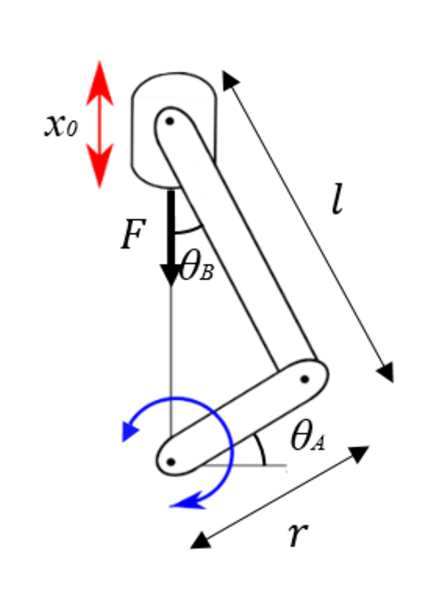
\includegraphics[height=50mm]{figure/slider_crank.eps}
    \vspace*{3mm}
    \caption{Slider Crank Mechanism}
    \label{fig:slider_crank}
  \end{center}
\end{figure}
% \vspace*{5mm}
% \begin{figure}[htp]
%   \begin{center}
%     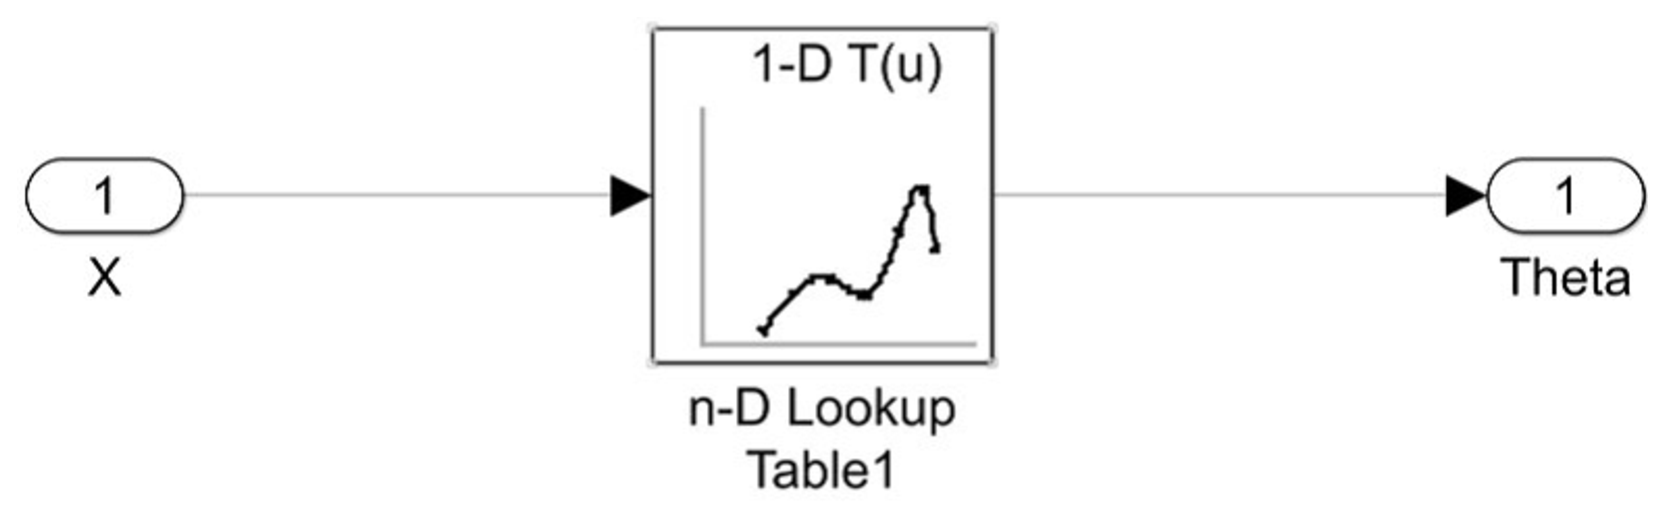
\includegraphics[height=30mm]{figure/Lookuptable.eps}
%     \vspace*{3mm}
%     \caption{Loou up table}
%     \label{fig:Look}
%   \end{center}
% \end{figure}

\subsubsection{計測機器}
本試験ではダンパが発生させるサスペンションストロークを計測する.ここでは計測に用いるロードセルとレーザ変位計について説明する.

まず,ロードセルについて説明する.ダンパが発生する力の計測には図~\ref{fig:tclz-20na}に示す東京測器研究所の引張・圧縮型高精度荷重計「TCLS-20NA」を用いた.仕様を表~\ref{tab:tclz_20na}~に示す.このロードセルをダンパとばね上の間に取り付けることでダンパ力を計測する.ロードセルから出力された電圧値は,東京測器研究所のデジタル指示計「TD-96A」を用いて寒山する.このデジタル指示計は,ひずみゲージ式変換器を用いて荷重,変位,圧力などを測定できる.外観を図~\ref{fig:td_96a}~に,仕様を表~\ref{tab:td_96a}~に示す.


\vspace*{10mm}
\begin{figure}[h!]
  \begin{tabular}{cc}
  \begin{minipage}{0.5\hsize}
  \begin{center}
    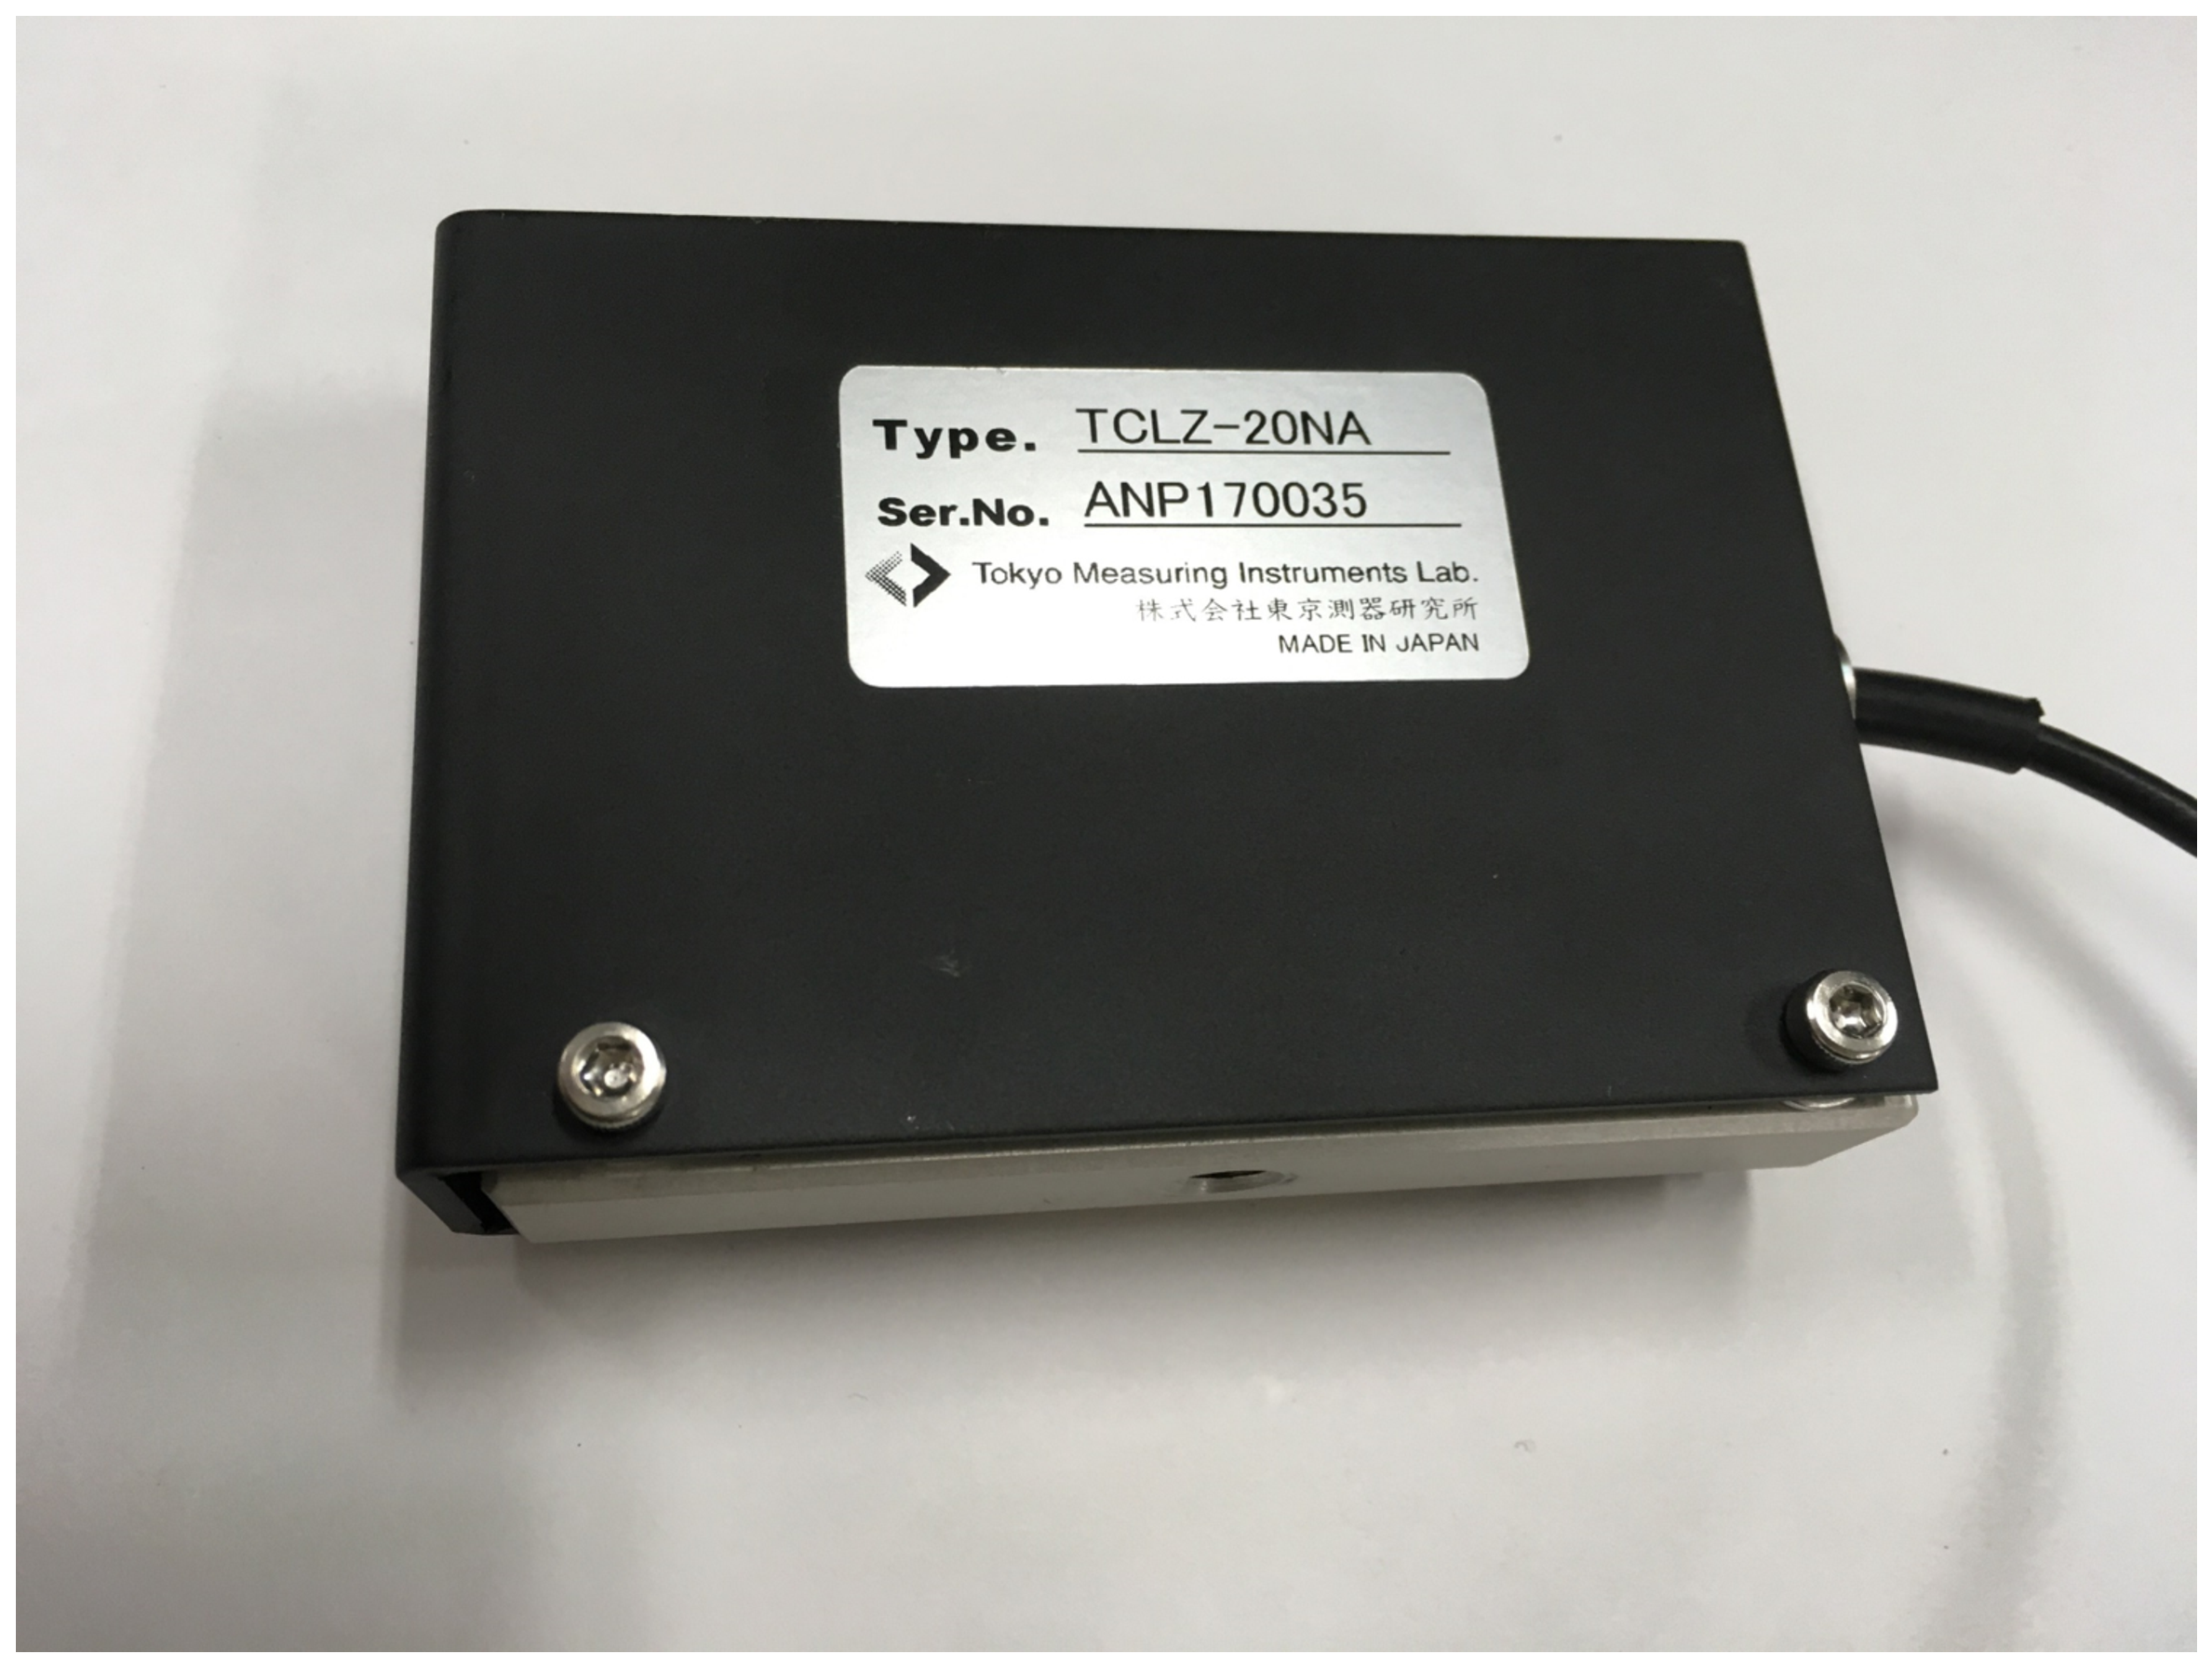
\includegraphics[height=40mm]{figure/tclz_20na.eps}
      \vspace*{3mm}
      \caption{Loadcell(TCLZ-20NA)}
      \label{fig:tclz-20na}
    \end{center}
  \end{minipage}
  \begin{minipage}{0.5\hsize}
     \begin{center}
      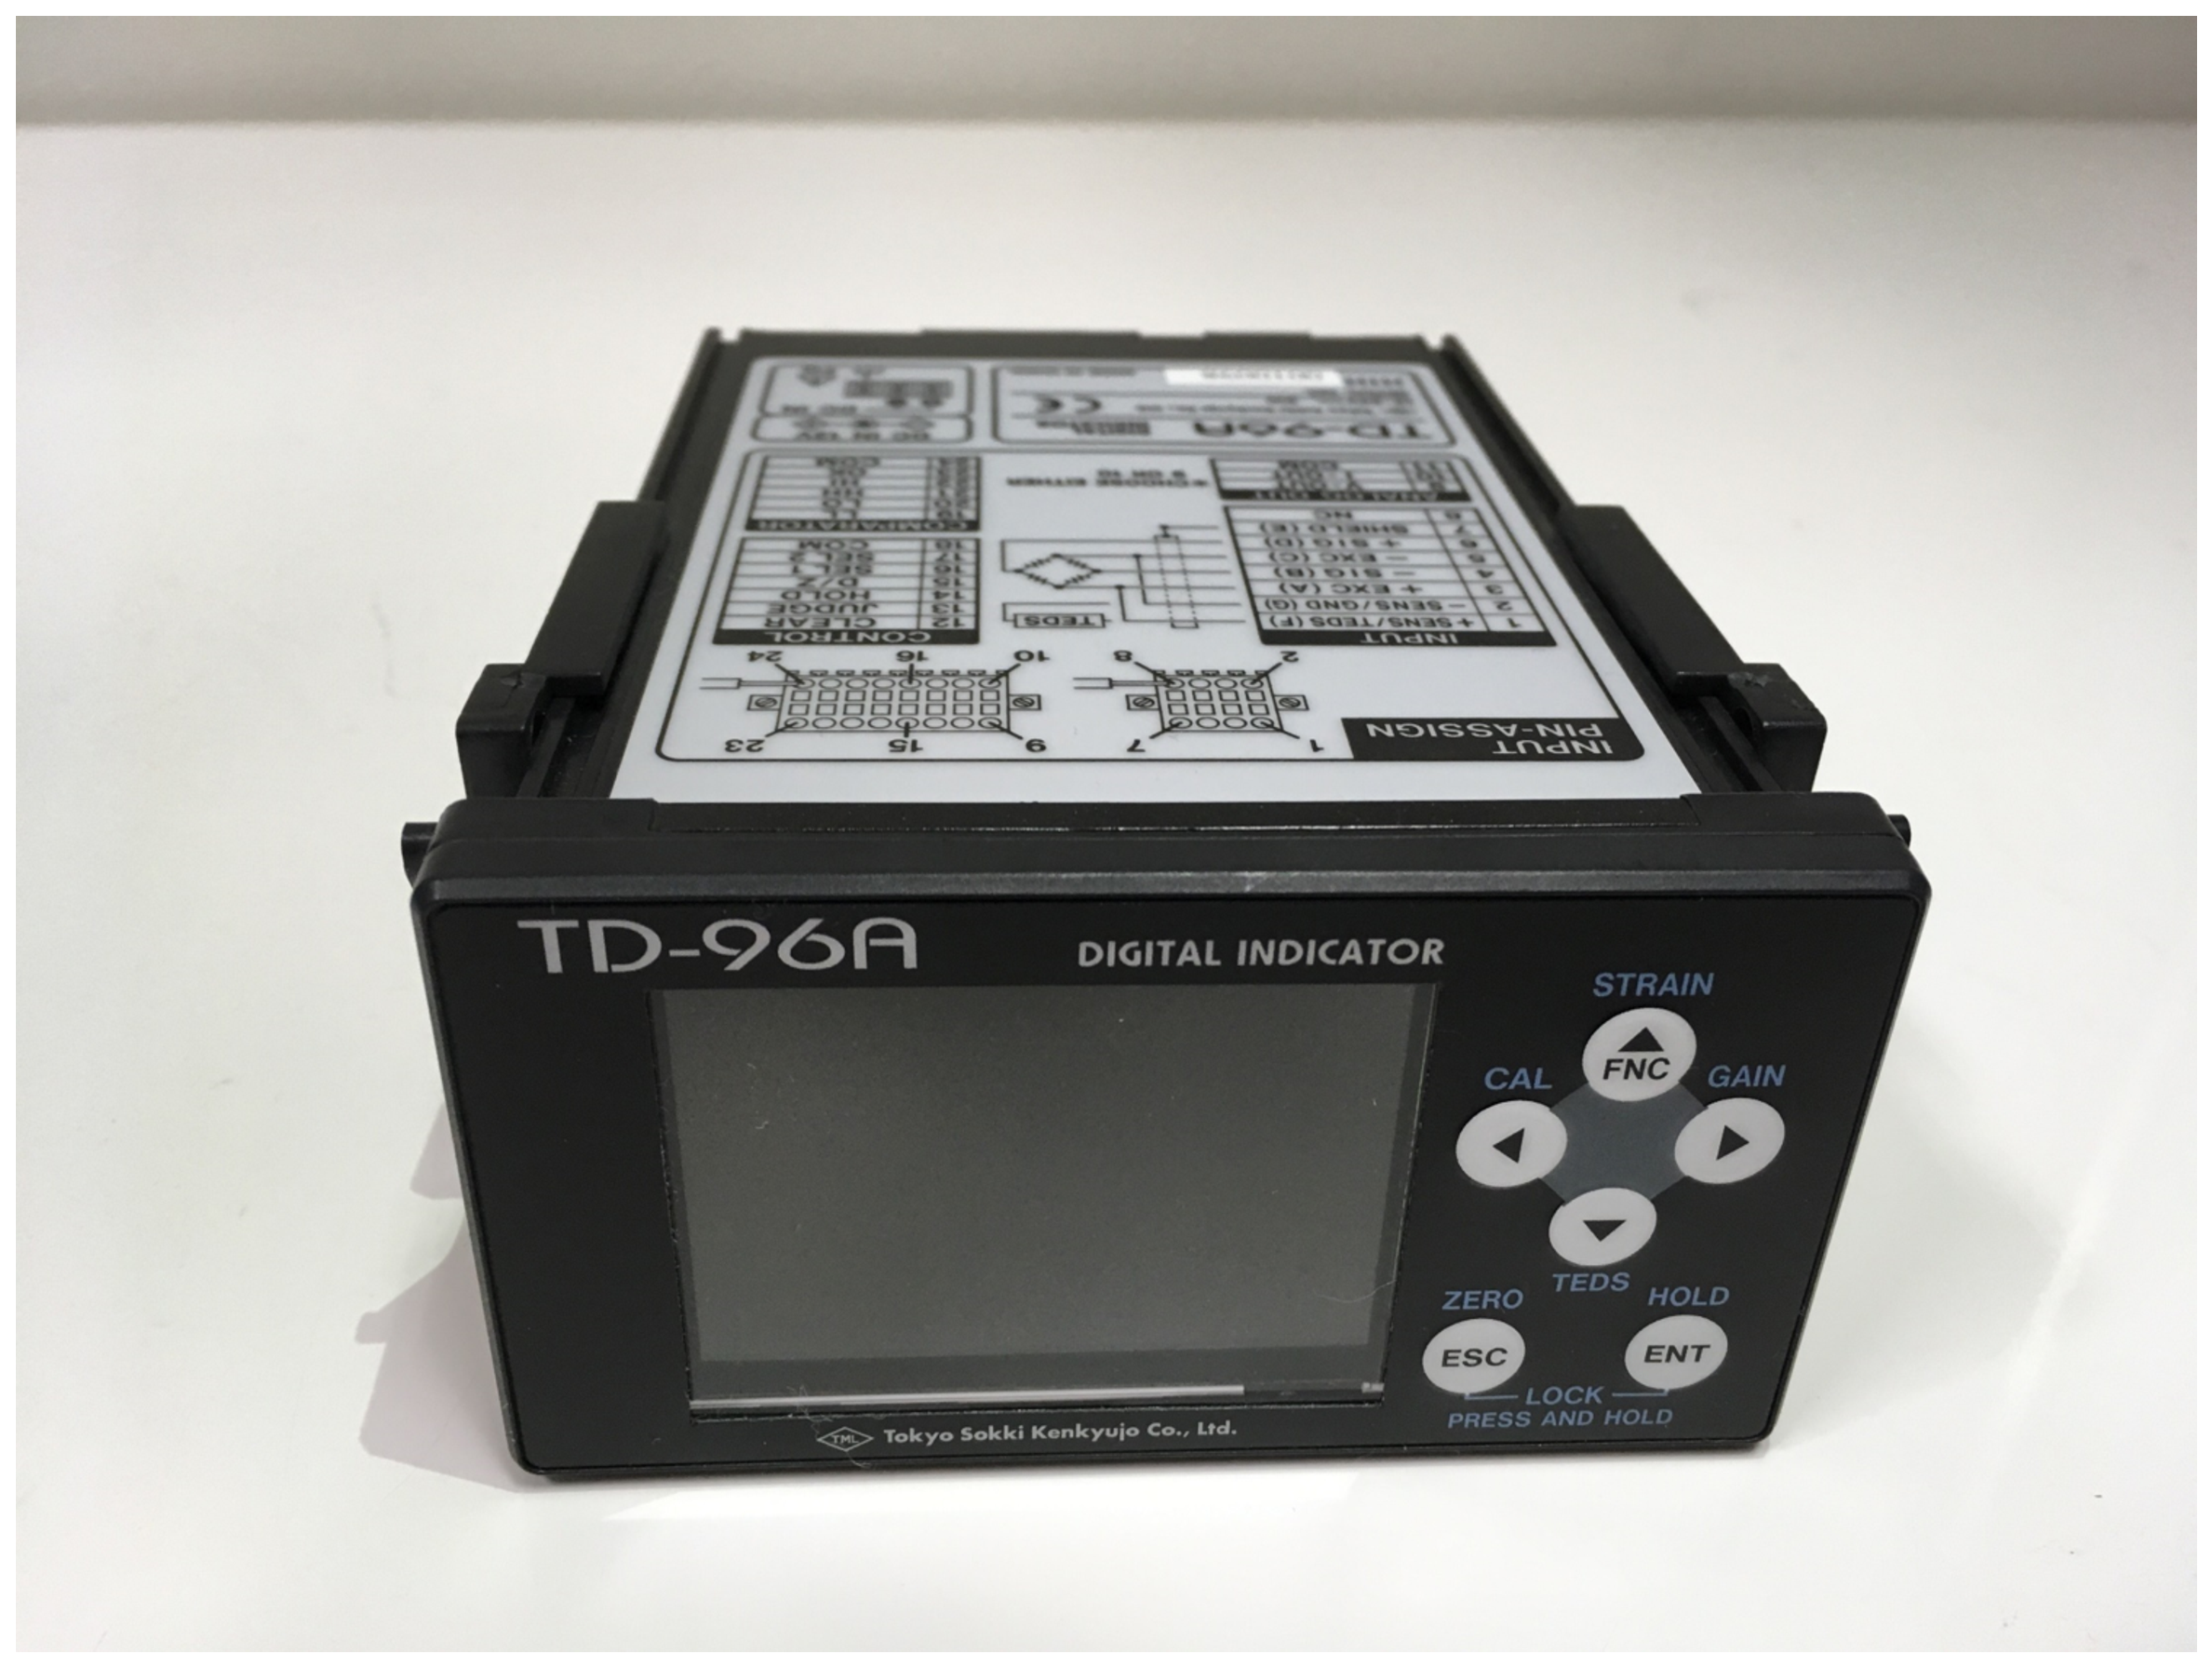
\includegraphics[height=40mm]{figure/td_96a.eps}
      \vspace*{3mm}
      \caption{Digital Indictor(TD-96A)}
      \label{fig:td_96a}
    \end{center}
  \end{minipage}
  \end{tabular}
 \end{figure}

\vspace*{10mm}
\begin{table}[h]
  \begin{center}
    \caption{Specification of Loadcell}
	\label{tab:tclz_20na}
	\begin{tabular}{crrc}\hline
	  Parameter & \multicolumn{2}{c}{Value}&\\\hline
	  Capacity & \multicolumn{2}{c}{20 N}&\\
	  Overload Capacity & \multicolumn{2}{c}{30N}&\\
	    & Ten.&Comp.\\
	  Rated Output & +1248.7 & -1248.4 & $\mu$V/V \\
	  Strain & +2497.3 & -2496.8 & $\times$ 10$^-6$ $\epsilon$ \\
	  Calibration Coefficient & 0.008009 & 0.008010 & N/1$\times$ 10$^-6$ \\\hline
	\end{tabular}
  \end{center}
\end{table}

\vspace*{10mm}
\begin{table}[h]
  \begin{center}
    \caption{Specification of TD-96A}
    \label{tab:td_96a}
    \begin{tabular}{cc}\hline
      Measurement Point & 1 \\
      Measurement Range [mV/V]& $\pm$3\\
      A/D Conversion Speed [Hz]& 4000\\
      D/A Output [mA]& 0$\pm$1$\sim\pm$10 V, 4$\sim$20\\
      Power supply & AC100 V 12 W, DC12$\sim$24 V 9 W \\\hline
    \end{tabular}
  \end{center}
\end{table}

\newpage
つづいてレーザ変位計について説明する.サスペンションストロークの計測には図~\ref{fig:il_300}~に示す株式会社KEYENCEのセンサヘッド「IL-300」を用いた.仕様を表~\ref{tab:il_300}~に示す.出力電圧は$\pm 5V,1-5V,0-5V$から選択できる.計測距離を$L[mm]$,アナログ出力電圧を$V[V]$としたとき,寒山式はそれぞれ以下の式のようになる.本研究では出力電圧$\pm 5V$の式(~\ref{eq:v5}~)を用いた.また,アンプとして,図~\ref{fig:il_1500}にに示す株式会社KEYENCEのアンプユニット「IL-100」を用いた.アンプユニットには,図~\ref{fig:lxo18_2a}~に示す定電圧/定電流直流電源「LXO18-2A」を用いて12Vをアンプユニットに供給している.

\begin{eqnarray}
 \label{eq:v5} L &=& V_{\pm5V} \times 28\\
 \label{eq:v15} L &=& V_{1-5V} \times 70\\
 \label{eq:v05} L &=& V_{0-5V} \times 56
\end{eqnarray}

\vspace*{10mm}
\begin{figure}[htp]
  \begin{minipage}{0.3\textwidth}
    \begin{center}
      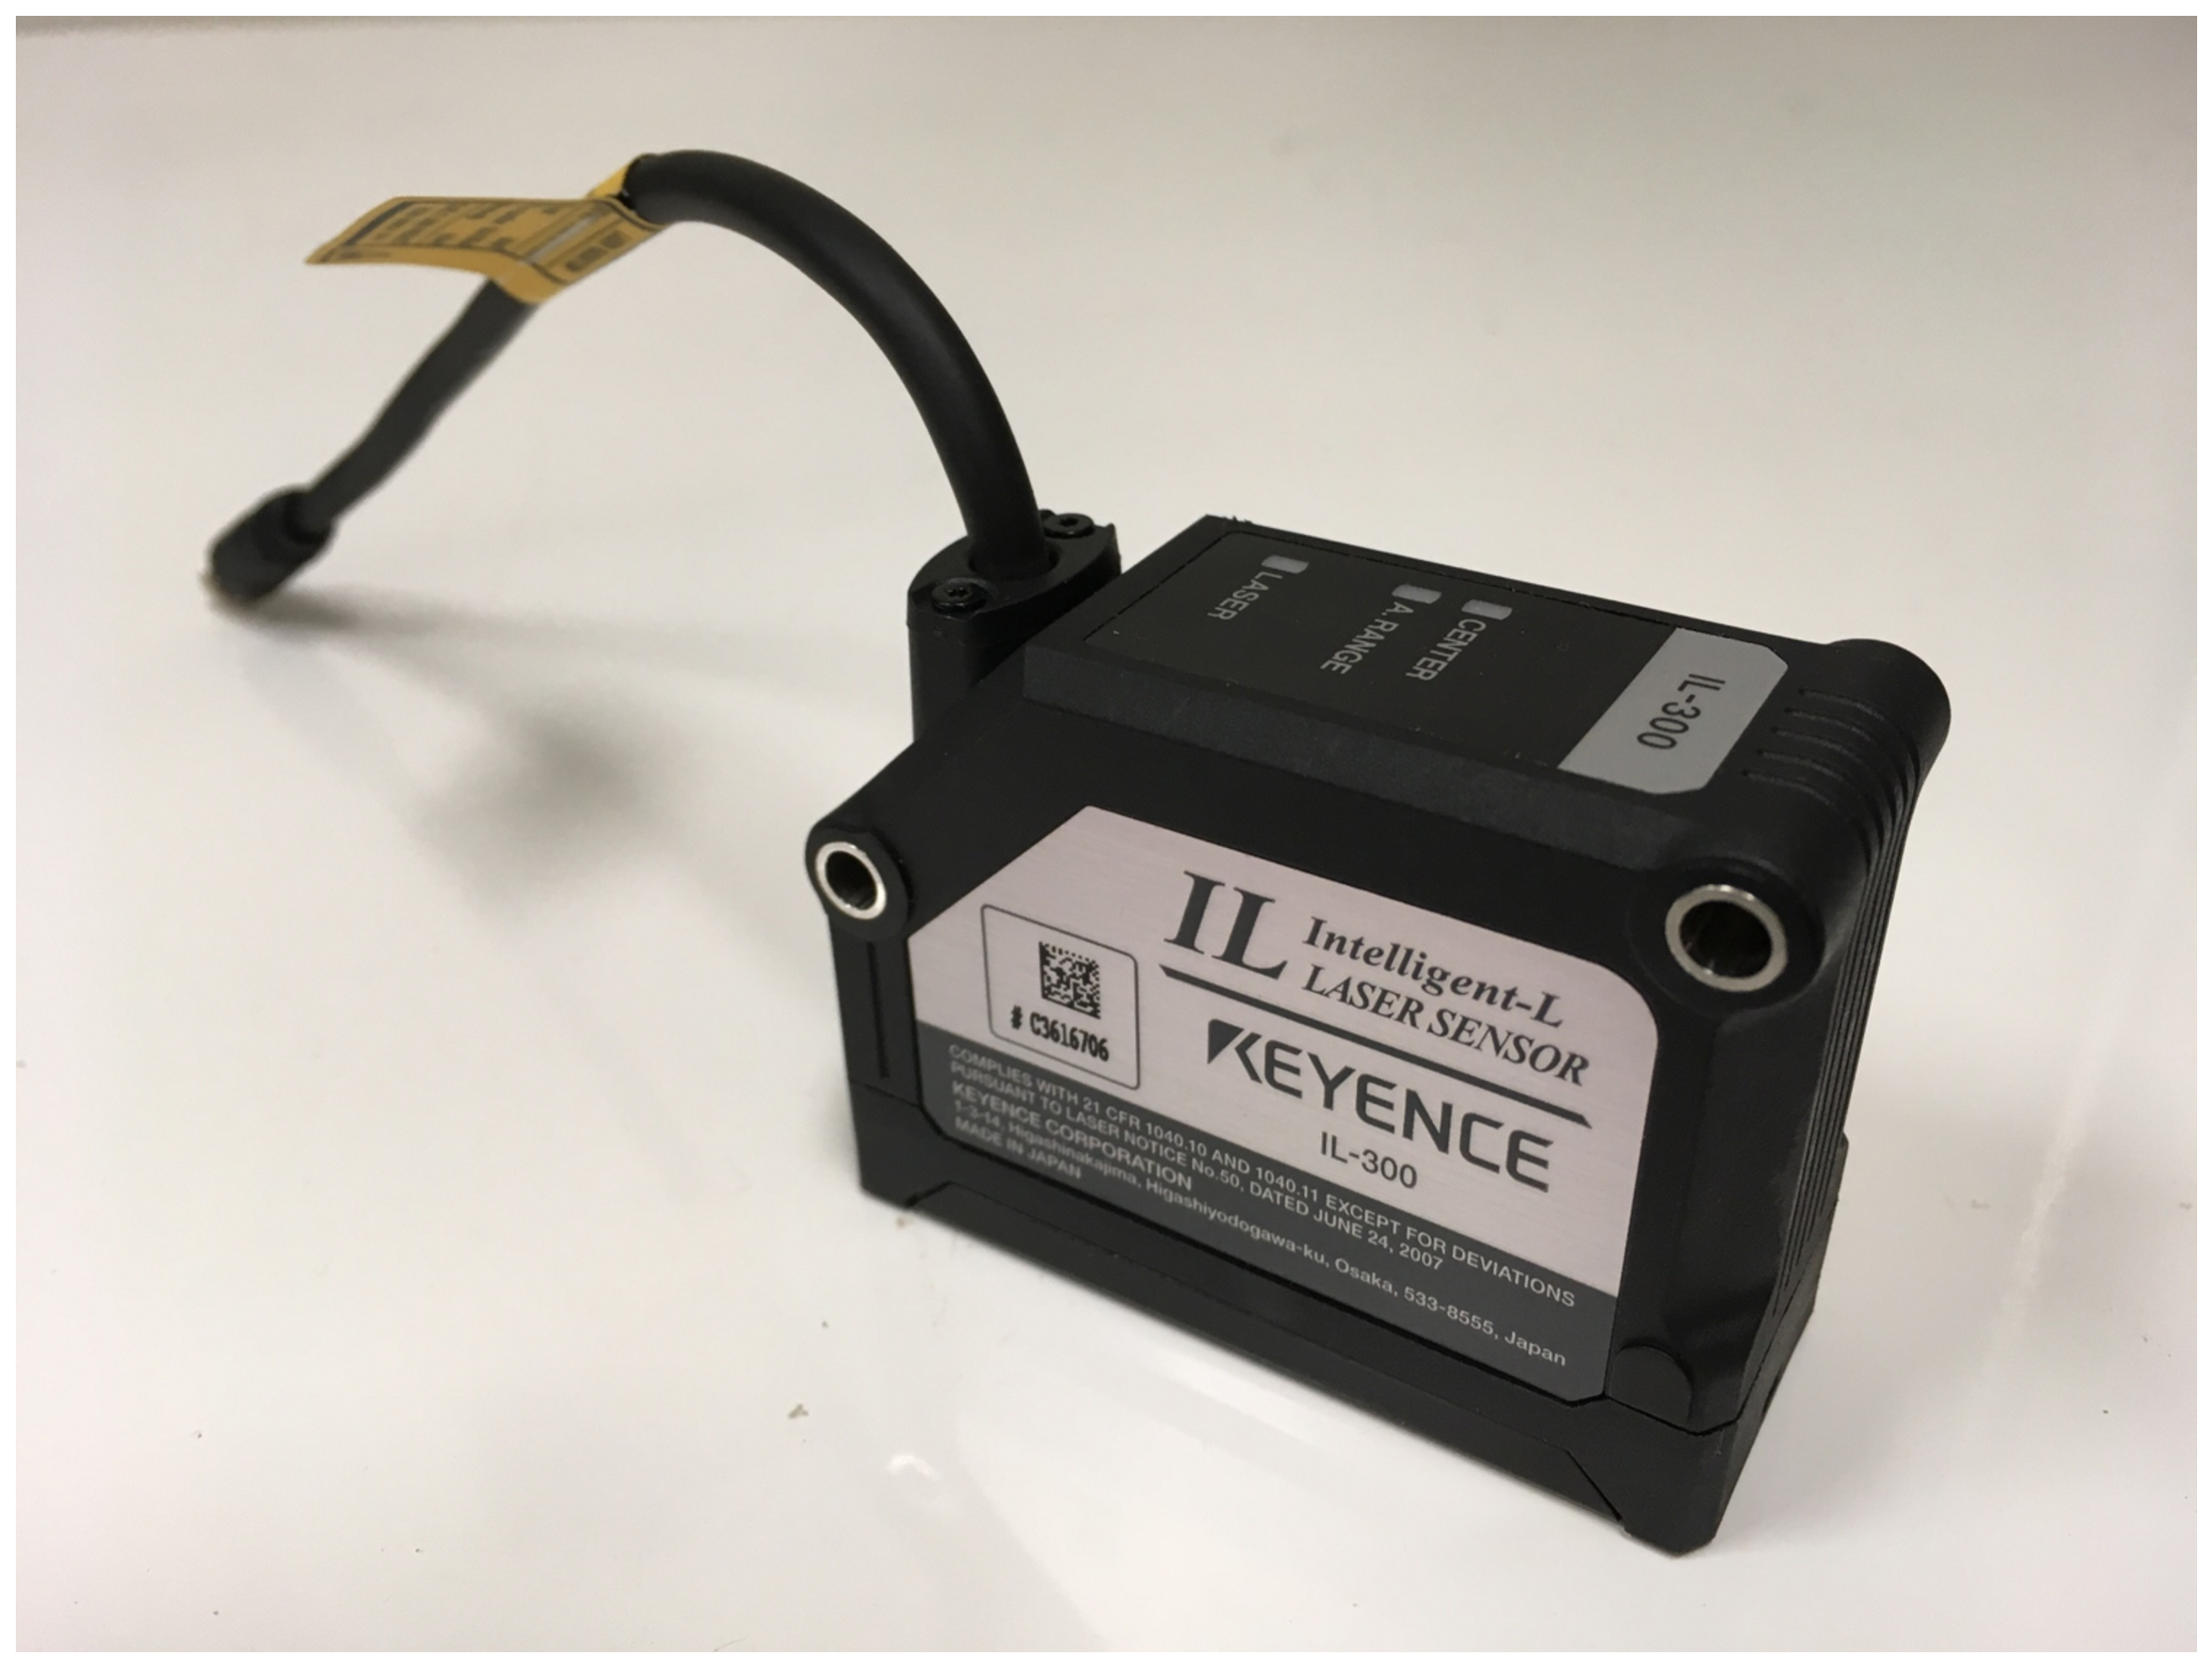
\includegraphics[height=40mm]{figure/il_300.eps}
      \vspace*{3mm}
      \caption{Laser Displacement Sensor(IL-300)}
      \label{fig:il_300}
    \end{center}
  \end{minipage}
  \begin{minipage}{0.7\textwidth}
      \begin{center}
	\makeatletter
	\def\@captype{table}
	\makeatother
	\caption{Specification of Laser Displacement Sensor}
	\label{tab:il_300}
	\begin{tabular}{ccc}\hline
	  Measurement Center Distance [mm] & 300\\
	  Measuring Range & 160-450 mm\\
	  Sampling Period [$\mu$s]& 0.33 / 1 / 2 / 5\\
	  Resolition [$\mu$m] & 10\\
	  Linearity [\%F.S.] & $\pm$0.25\\
	  Receiving Element & Liner Image Sensor\\
	  Resistance to Vibration [Hz] & 10-55\\
	  Laser Class & 2\\
	  Power Supply & DC10-30 V\\\hline
	  \end{tabular}
	\end{center}
  \end{minipage}
\end{figure}

\vspace*{10mm}
\begin{figure}[htp]
  \begin{minipage}{0.5\textwidth}
    \begin{center}
      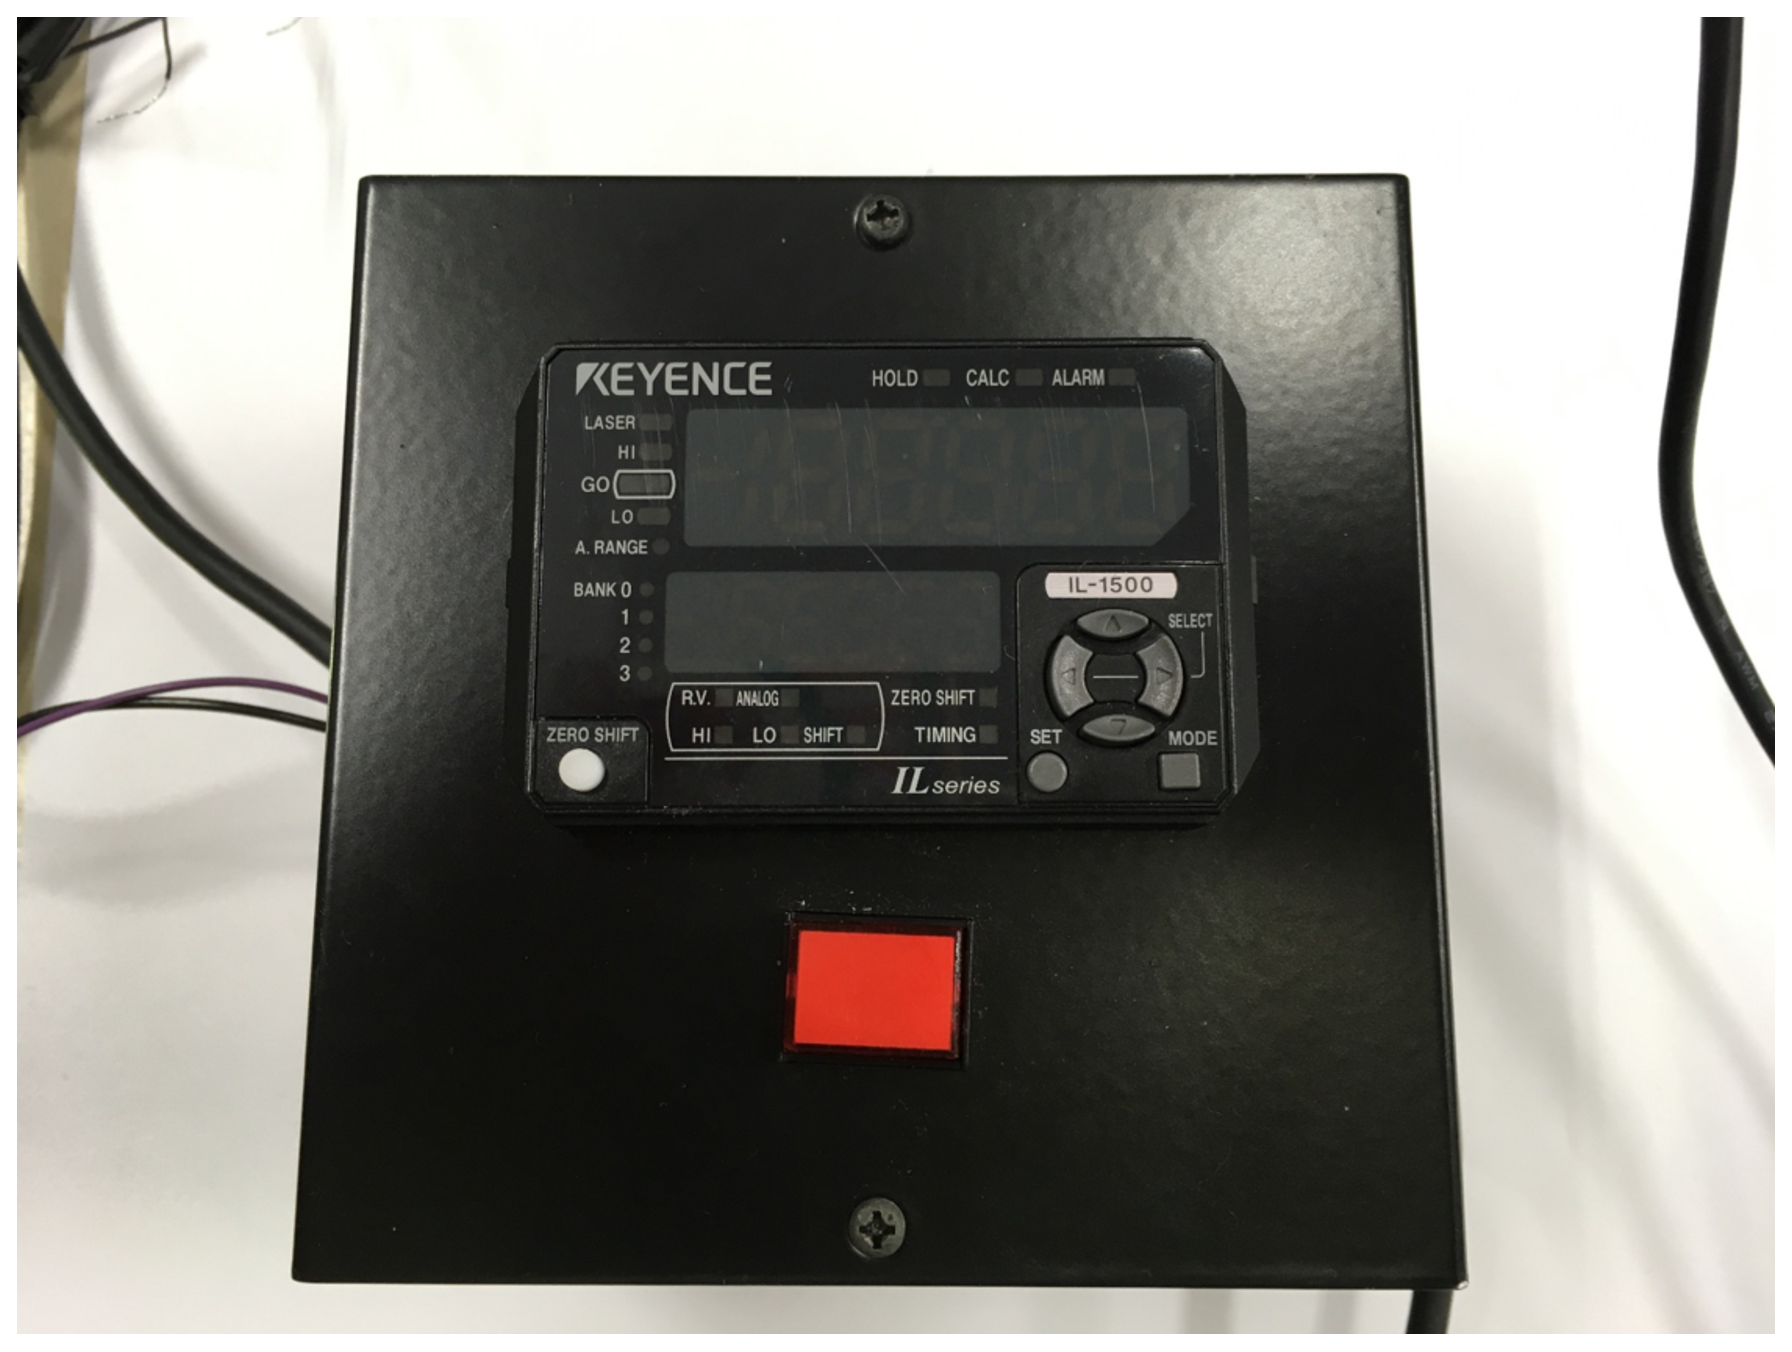
\includegraphics[height=40mm]{figure/il_1500.eps}
      \vspace*{3mm}
      \caption{Amplifier Unit(IL-1000)}
      \label{fig:il_1500}
    \end{center}
  \end{minipage}
  \begin{minipage}{0.5\textwidth}
    \begin{center}
      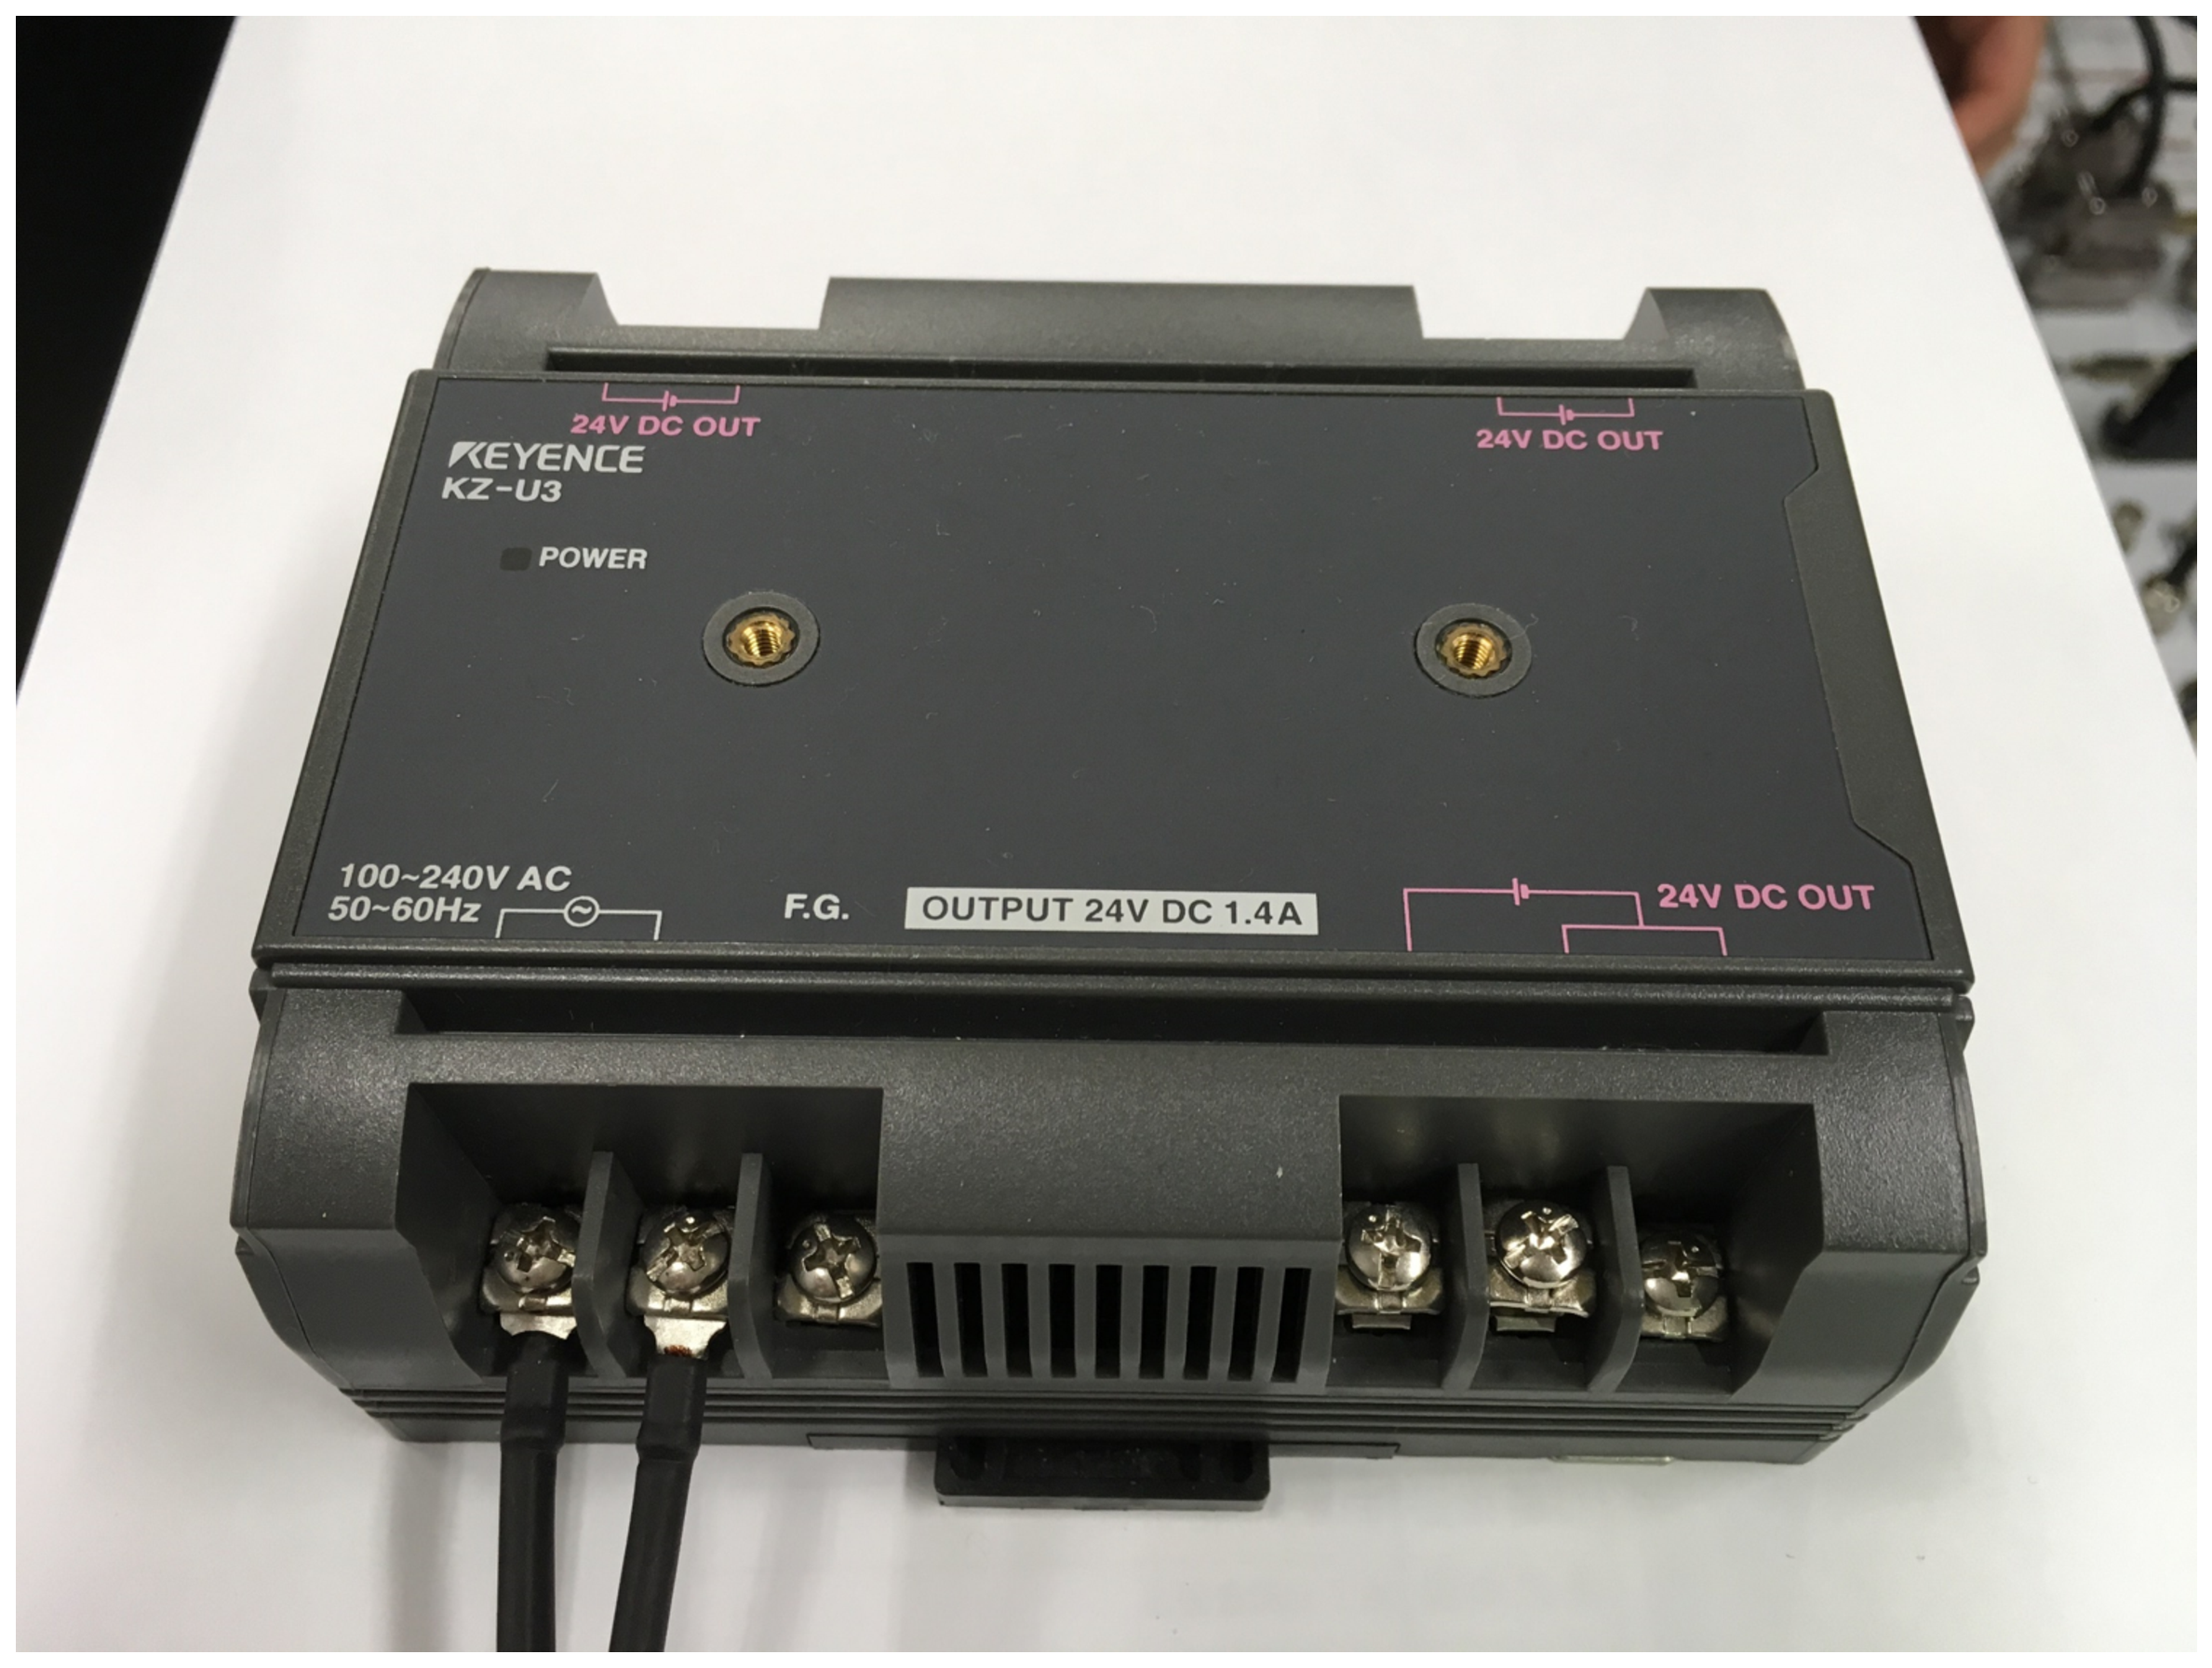
\includegraphics[height=40mm]{figure/lxo18_2a.eps}
      \vspace*{3mm}
      \caption{Power Supply Unit(LXO18-2A)}
      \label{fig:lxo18_2a}
    \end{center}
  \end{minipage}
\end{figure}




\newpage
\begin{thebibliography}{99}
\bibitem{pic_sus.net}https://nge.jp/wp-content/uploads/2015/08/shutterstock\_22066612.jpg
\bibitem{exp_hils1}永井正夫,吉田秀久,Noomwongs Nuksit,横井隆,川眞田智,小林克宏,タイヤHIL シミュレータによる車両運動性能の研究(第1報) : タイヤHIL シミュレータの開発,自動車技術会論文集,Vol35,No.2,(2004),pp.147-152
\bibitem{exp_hils2}山口輝也, 実ヨーダンパを用いたHardware-In-the-Loopシミュレーションによる鉄道車両の蛇行動安定性試験(試験環境の構築と安定的な検証), 日本機械学会論文集,C編Vol.79 No.806(2013-10),pp.131-142
\bibitem{toyota_hils}https://www.toyota.co.jp/jpn/company/history/75years/data/automotive\_business/ \\ products\_technology/technology\_development/performance/images/supplement\_img01.jpg

\bibitem{daisyarin}大車林,三栄書房,(2003)
\bibitem{thesis_airpot}Keita Koumo, Naoto Abe, Taichi Matsuoka, Switching Control based on the mode of vibration for Dynamic Absorber, IEEE Control Conference (ASCC), 2015 10th Asian
\bibitem{picture_airpot}$\rm{http://www.airpot.jp/airpot.html}$
\bibitem{asami}浅見 敏彦,関口 久美,空気ダンパの基礎的研究(第1報, 理論解析),日本機械学会論文集(C編),56巻526号(1990-6)
\bibitem{nasu}浅見 敏彦,横田 泰孝,伊勢 智彦,本田 逸郎,坂本 博哉,オリフィス付き空気ばねの非線形特性解析と実験による検証,日本機械学会論文集(C編),77巻777号(2011-5)
\bibitem{shiiba}浅見 敏彦,粘性減衰の利用,公益社団法人 日本騒音制御工学会,騒音制御,1994 年 18 巻 3 号 p. 120-125
\bibitem{dspace}$\rm{http://www.dspace.com/ja/jpn/home.cfm}$
\bibitem{maxon}$\rm{http://academy.maxonjapan.co.jp/mmc}$
\bibitem{99}http://github.com/ethz-asl/matlab\_epos\_library
\end{thebibliography}

\end{document}
